
\def\thudbabelopt{english,italian}
\documentclass[target=mst]{thud}
\usepackage{graphicx}
\usepackage{float}

\title{Relazione del Laboratorio \\ di Deep Learning, \\ Emotions Recognition}
\author{Zuccato Francesco 143095 \\ \ Bolletta Christian 142478}
\phdnumber{313}
\cycle{XXVIII}




\usepackage[a-1b]{pdfx}
\usepackage[pdfa]{hyperref}

%% due colonne
\usepackage{multicol}
%% manage images
\usepackage{graphicx}
\usepackage{wrapfig}
\usepackage{float}
\usepackage[rightcaption]{sidecap}
\graphicspath{ {./images/} }
\usepackage{caption}
\usepackage{subcaption}
\captionsetup[figure]{font=small, labelfont=small} %%options: scriptsize, footnotesize, small, normalsize, large, Large

\begin{document}
\maketitle

\abstract
In questo laboratorio è richiesto di realizzare una rete neurale in grado di predire le emozioni dal database "fer2013.csv" che contiene 35887 immagini di 48x48 pixel.
Nello specifico, in ogni riga è presente sia un'immagine in bianco e nero della faccia di una persona, sia la relativa emozione, compresa tra le seguenti: rabbia, disgusto, paura, felicità,  tristezza, stupore, neutralità.

Per l'analisi di immagini è noto come le reti più adatte siano le CNN (\textit{Convolutional Neural Networks}).
Nel testo è presentata il preprocessing e l'analisi iniziale del dataset, l'implementazione di alcuni modelli di CNN e l'analisi dei risultati finali.

%% Indice
\tableofcontents

%% Lista delle tabelle (se presenti)
%\listoftables

%% Lista delle figure (se presenti)
%\listoffigures

%% Corpo principale del documento
\mainmatter

%% Parte
%% La suddivisione in parti è opzionale; solitamente sono sufficienti i capitoli.
%\part{Parte}

%% Capitolo
\chapter{Analisi e Preprocessing del dataset}

%% Sezione
%\section{Analisi}

\begin{wrapfigure}{r}{0.4\textwidth}
  \label{EmotionsCount}
  \centering
  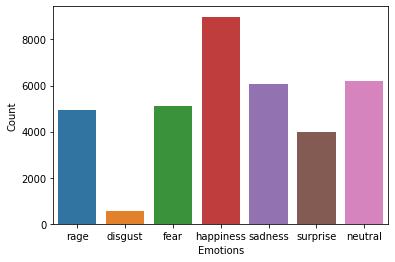
\includegraphics[width=0.4\textwidth]{EmotionsCount.png}
  \caption{Numero di campioni per emozione}
  %%\vspace{-20pt}
\end{wrapfigure}

Il dataset è formato da immagini, ciò implica che non è possibile eseguire un'analisi iniziale delle \textit{x}. Non resta che analizzare le \textit{y} del dataset, ovvero le emozioni. Si è contato il numero di campioni per emozione, ed è emerso che non è presente una distribuzione uniforme delle labels. 

Dal grafico si può vedere come siano presenti pochissimi campioni per il disgusto, e, di conseguenza, tale emozione sara molto più difficilmente apprendibile nella fase di riconoscimento. 
Al contrario, la felicità sarà l'emozione su cui predire sarà più semplice e si otterrà un'accuracy migliore.


%\begin{center}
%\includegraphics[scale=0.5]{trasferimento.png}
%\end{center}
 
\subsubsection{Divisione in Train, Validation, Test }
Sebbene nel dataset sia già fornita una possibile suddivisione del dataset è stato deciso comunque di eseguire uno split randomico, specificando l'opzione \textit{stratify=y}, per non alterare le distribuzioni delle \textit{y}.

La dimensione del train usata è il classico 70\%, ovvero 25120, che è un po' più piccola del 28709, che è quella consigliata.
L'utilizzo del random split evita il rischio di focalizzarsi solo su una parte dei dati, e, memorizzando ed esportando il random seed usato, si garantisce la riproducibilità delle divisioni.

\subsubsection{Preprocessing}
Dall'analisi è risultato quindi che il dataset contiene un numero abbastanza esiguo di campioni, circa 35mila, e non è uniformemente distribuito.
Si è deciso di procedere con l'\textit{augmentation} delle immagini. Tale procedura consente di "ingrandire" un database col fine di ottenere più informazioni necessarie per l'addestramento della rete. 

Per il caso delle immagini si possono utilizzare varie tecniche, modificando sia le coordinate spaziali dei pixels, tramite rotazioni, inversioni, ritagli ecc., sia i colori, facendo uso di appositi filtri. Tra questi si annoverano l'\textit{edge-detector}, per la rilevazione le righe verticali e/o orizzontali, il \textit{sobel} per i contorni, ed altri ancora per modificare contrasto, luminosità ed intensità dei colori.

Per non appesantire troppo la rete, è stato deciso di fare uso di solamente due filtri: il sobel e uno per l'aumento del contrasto, entrambi aggiunti al dataset chiamato 'fer2021.csv', usato poi nella rete.


\chapter{Rete CNN}
La rete è stata implementata in modo parametrico, così da agevolare la modifica dei parametri quali il numero di layers, le dimensioni dei pesi ed il numero dei canali.
Per fare ciò sono state realizzate due reti diverse, entrambe parametriche.
Le reti sono generate dinamicamente a tempo di compilazione, in quanto la grandezza delle liste e degli output sono passati alla rete stessa come parametri.

\begin{multicols}{2}

\noindent
1) una lista di (n liste di \textit{CDrop-Block}, \textit{MaxPool2D}) \\%, formati da \textit{Conv2D}, \textit{DropOut}, \textit{ReLU}\\
2) un \textit{DropOut}\\
3) una lista di \textit{Linear}\\
4) una \textit{SoftMax}

\columnbreak

\noindent
1) una lista di (n liste di \textit{C-Block}, \textit{MaxPool2D}) \\%, formati da \textit{Conv2D}, \textit{ReLU}\\
2) un \textit{DropOut}\\
3) una lista di \textit{Inception-Block} \\%, realizzati come da specifiche Google \\
        %(con la possibilità di aumentare la dimensionalità degli output)
4) un \textit{DropOut}\\
5) una lista di \textit{Linear}\\
6) una \textit{SoftMax}
\end{multicols}

% toooo much space
%\begin{enumerate}
%    \item una lista di \textit{Conv-Block}, formati da \textit{Conv2D}, \textit{DropOut}, \textit{ReLU}
%    \item una lista di \textit{Linear}
%    \item una \textit{SoftMax}
%\end{enumerate}
%\\La seconda:
%\begin{enumerate}
%    \item una lista di \textit{Conv-Block}, formati da \textit{Conv2D}, \textit{ReLU}
%    \item un \textit{DropOut}
%    \item una lista di \textit{Inception}, realizzati come da specifiche Google 
%        %(con la possibilità di aumentare la dimensionalità degli output)
%    \item un \textit{DropOut}
%    \item una lista di \textit{Linear}
%    \item una \textit{SoftMax}
%\end{enumerate}

\section{Convolutional Part}

\begin{figure}[h!]
    \centering
    %\advance\leftskip2.25cm
    % start
    \begin{minipage}[b]{0.4\textwidth}
      \centering
      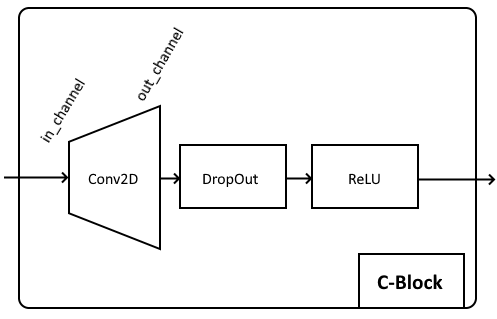
\includegraphics[scale=0.455]{ConvDrop-Block.png}
      \caption{ConvDrop-Block}
      \label{fig:ConvDrop-Block}
    \end{minipage}
    % mid
    \begin{minipage}[b]{0.4\textwidth}
      \centering
      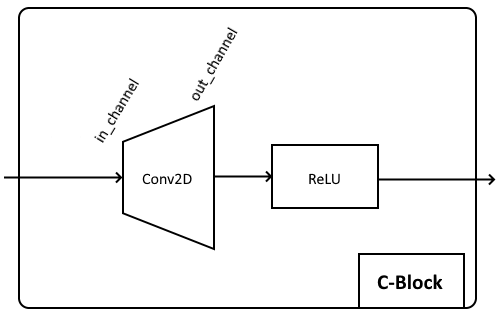
\includegraphics[scale=0.455]{Conv-Block.png}
      \caption{Conv-Block}
      \label{fig:Conv-Block}
    \end{minipage}
    % end
\end{figure}

\noindent
La parte convoluzionale è composta da una sequenza di blocchi (Fig. \ref{fig:SequenceOfC-Block}) che vengono ripetuti un $a_0$ volte, poi sono filtrati da un MaxPool, poi si ripetono di nuovo $a_1$ volte, poi filtrati da un MaxPool ecc.
Solitamente il numero dei blocchi esterni usato è 3-5, la ripetizione di ciascun blocco interno è 1-4 volte.

I blocchi esterni sono così implementati: il primo blocco interno riceve $in\_chan=3=N_0$ e produce $out\_chan=N_1$, i seguenti blocchi interni continuano a produrre canali grandi $N_1$.
Poi c'è il MaxPool e quindi il secondo blocco esterno, in cui il primo interno incrementerà i canali da $N_1$ a $N_2$ ecc.

Si noti come sia possibile (ma non avrebbe molto senso) diminuire le dimensioni dei canali. Ciò che invece dimuinuisce dopo ogni blocco esterno è la dimensione dell'input, che viene dimezzato dal MaxPool2D (ma che preserva la dimensione dei canali).
Ogni blocco interno (Fig. \ref{fig:ConvDrop-Block}, \ref{fig:Conv-Block}) è composto da un Conv2D, un DropOut (nel caso 1) e da una ReLU.

\begin{figure}[H]
    %\advance\leftskip1.5cm
    \centering
    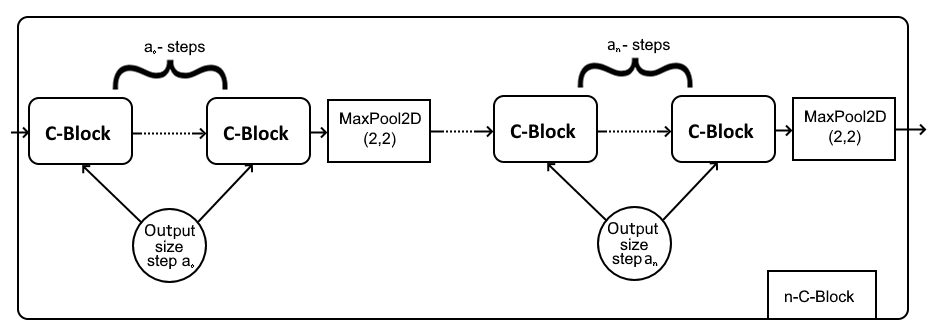
\includegraphics[scale=0.6]{SequenceOfC-Block.png}
    \caption{Lista di (lista di C-Block, MaxPool)}
    \label{fig:SequenceOfC-Block}
\end{figure}

\subsection{Inception Part}
Per migliorare la stabilità e non ottenere un alto livello di overfit si è deciso di implementare una sequenza di Inception. Sono implementati come da specifiche Google, con una generalizzazione.
La versione originale prevede infatti 256 canali di output: 64 da 1x1, 128 da 3x3, 32 da 5x5, 32 da pool. Mentre il codice prevede un parametro \textit{incep\_\_multiplier} che consente di ritornare $256 * mul$ canali.

Solitamente \textit{mul} è stato usato con valori pari a 1 (ininfluente), ma soprattutto con 2 ($out\_ch=512$) o 3 ($out\_ch=769$).
Si è evidenziato come l'aggiunta degli inception modules in gran numero (da 15 a 30) garantisca molta stabilità alla rete ed una crescita lenta ma abbastanza costante, al contrario un numero ridotto è praticamente inutile, soprattutto in un dataset piccolo come quello in questione.

\begin{figure}[h!] 
  \centering
  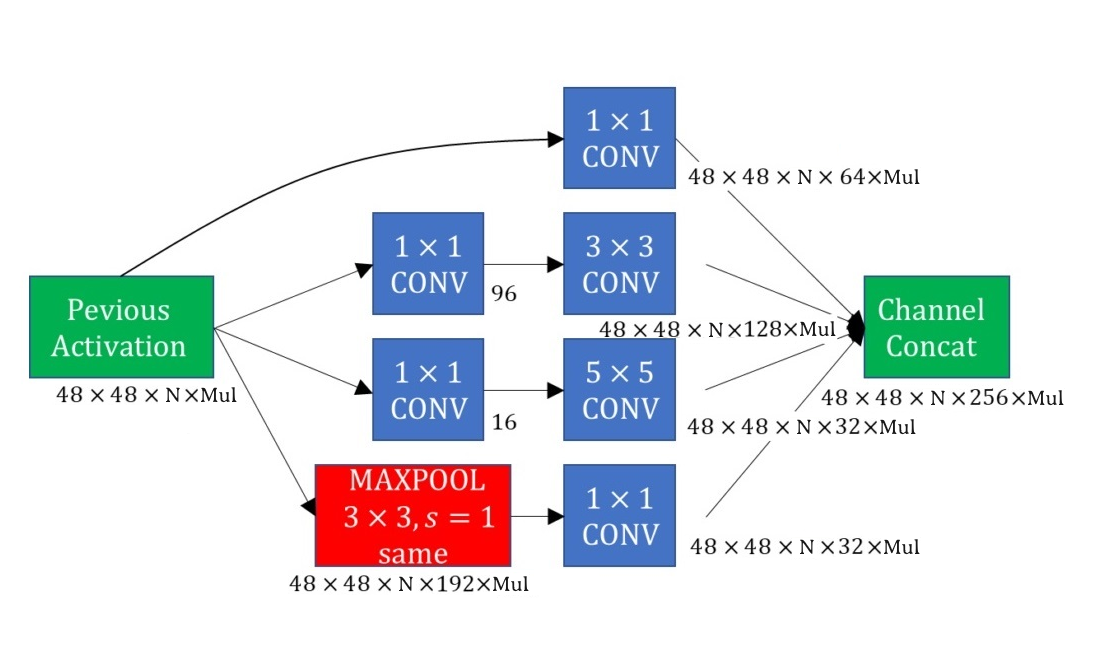
\includegraphics[scale=0.45]{inception.png}
  \caption{Inception Module}
  \label{fig:Inception}
\end{figure}
\vfill

\subsection{Classification Part}
La parte di classificazione (Fig. \ref{fig:linear}), anch'essa parametrica, consiste in un susseguirsi di Linear layers di dimensione decrescente, fino all'ultimo che avrà dimensione pari a 7, che è il numero delle label. 
Questo diventa poi l'input per la SoftMax che finalmente restituirà la predizione dell'emozione dell'immagine.
Solitamente in classificazione sono usati 4-5 layers, il primo con 500-1000 valori in input e i seguenti con un fattore decrescente esponenziale (1/2, 1/4, 1/8 del precedente).

\begin{figure}[h!]
  %\advance\leftskip4cm
  %\advance\rightskip-4cm
  \centering
  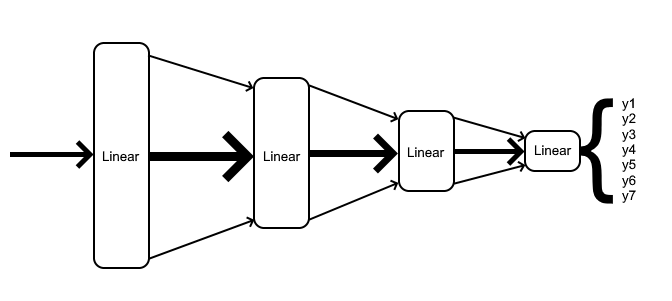
\includegraphics[scale=0.75]{SequenceOfLinear.png}
  \caption{Linear Layers}
  \label{fig:linear}
\end{figure}

\chapter{Analisi complessiva}
In questi giorni sono state provate molte reti diverse. Si è giunti alla conclusione che le migliori fossero quelle spiegate prima, senza moltissimi layer (dai 3 ai 8 solitamente) ma con canali di output molto grandi (ad es. 50,100,250,500), fino ad un massimo di 800, note come 'fat'. Entrambe le reti raggiungono il 50-60\% di accuracy in testing.
In ogni rete però il problema maggiore è quello di riuscire a riconoscere il disgusto, molte di quelle provate ottengono tutte lo 0\%.

\section{R1: Rete senza inceptions}
La rete senza gli inceptions ottiene un'accuracy in training decisamente più alta, il 75-85\%, rispetto a quella nel test, il 60\%. Ovviamente la rete è andata in overfit. 
Tuttavia, questa è la migliore realizzata per l'accuracy nel testing accuracy. Inoltre, come si vede dalla Confusion Matrix (Fig. \ref{fig:R1_confusion_matrix}) è in grado di riconoscere \textbf{tutte} le labels, compreso il disgusto.
Dalle osservazioni fatte usando parametri diversi si è riscontrato che le performance migliori si ottengano usando reti molto profonde e con pochi layers, mentre le reti "snelle" non producono un'accuracy accettabile (sopra il 50\%).
Il difetto principale di queste reti è sicuramente l'overfitting, che in certe osservazioni ha prodotto un'accuracy anche del 100\% (!) in training (mentre in testing del 55-60\%).
Siccome il DropOut2D utilizzato è del 35\% per contrastare l'overfitting è stato provato un dropout maggiore (40-50\%) ma il risultato è che l'accuracy si riduceva drasticamente.
A causa del trade-off e dei tempi di consegna ristretti abbiamo accettato un overfitting elevato che ci consente un buonissimo 60\% di accuracy in testing.

\section{R2: Rete con inceptions}
La rete con gli inceptions migliore ha ottenuto un'accuracy del 57\%.
Si è riscontrato essere più lenta nell'apprendimento ma ad avere un overfit minore.
Sicuramente sarebbe la rete ideale se il dataset fosse maggiore e se ci fosse stato il tempo di testarla con 100 epoche più volte, magari usando un learning rate minore ($1^{e-5}$ al posto di $1^{e-4}$) e con un dropout (forse) ancora maggiore del 62\%, attualmente usato.
Le prestazioni attualmente migliori le si sono ottenute concatenando ben 30 (!) inceptions modules diversi, con fattore moltiplicativo dei canali di output pari a 3.
Purtroppo nessuno dei vari tentativi con questa rete è stato in grado di riuscire a predirre il disgusto, sempre fermo allo 0\% di accuracy in testing.

%%CONFUSION MATRIX
\begin{figure}[h!]
    \centering
    %\advance\leftskip2.25cm
    % start
    \begin{minipage}[b]{0.48\textwidth}
      \centering
      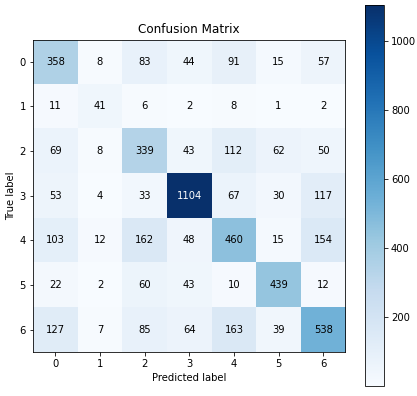
\includegraphics[scale=0.75]{R1_confusion_matrix.png}
      \caption{R1 confusion matrix}
      \label{fig:R1_confusion_matrix}
    \end{minipage}
    % mid
    \begin{minipage}[b]{0.48\textwidth}
      \centering
      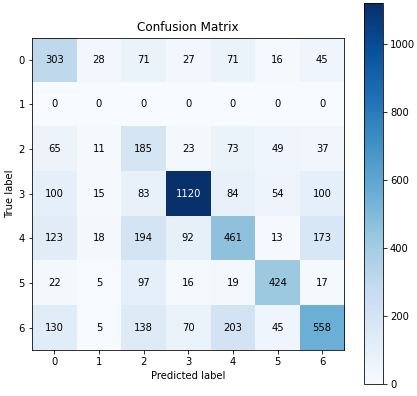
\includegraphics[scale=0.75]{R2_confusion_matrix.png}
      \caption{R2 confusion matrix}
      \label{fig:R2_confusion_matrix}
    \end{minipage}
    % end
\end{figure}

%ACCURACIES MATRIX  
\begin{figure}[h!]
    \centering
    %\advance\leftskip2.25cm
    % start
    \begin{minipage}[b]{0.48\textwidth}
      \centering
      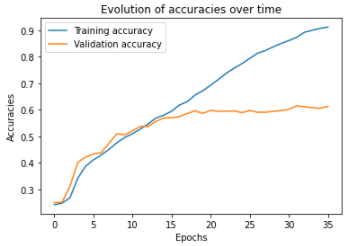
\includegraphics[scale=0.85]{R1_accuracy.png}
      \caption{R1 accuracy}
      \label{fig:R1_accuracy}
    \end{minipage}
    % mid
    \begin{minipage}[b]{0.48\textwidth}
      \centering
      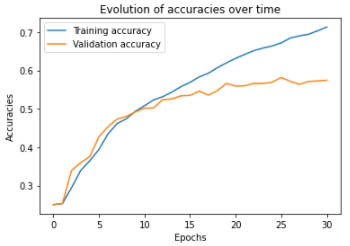
\includegraphics[scale=0.85]{R2_accuracy.png}
      \caption{R2 accuracy}
      \label{fig:R2_accuracy}
    \end{minipage}
    % end
\end{figure}

%%SUMMARY
\begin{figure}[h!]
    \centering
    %\advance\leftskip2.25cm
    % start
    \begin{minipage}[b]{0.48\textwidth}
      \centering
      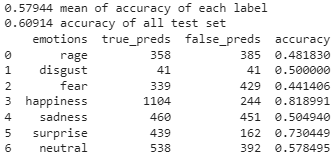
\includegraphics[scale=0.85]{R1_summary.png}
      \caption{R1 summary}
      \label{fig:R1_summary}
    \end{minipage}
    % mid
    \begin{minipage}[b]{0.48\textwidth}
      \centering
      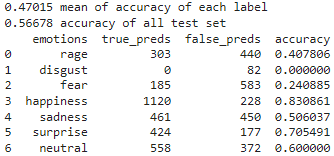
\includegraphics[scale=0.85]{R2_summary.png}
      \caption{R2 summary}
      \label{fig:R2_summary}
    \end{minipage}
    % end
\end{figure}


\chapter{Conclusione}
Dai i dati da noi analizzati, e dalle varie reti testate; sopraggiungiamo alla conclusione che le reti che fanno uso di Inception Modules sarebbero da usare su reti neurali molto più profonde e su dataset molto più popolati, così da consentirne una maggiore efficenza; mentre nel caso si volesse usufruire di reti meno profonde, dai nostri dati abbiamo concluso che le Pure Convolutional danno il meglio di loro nel caso siano molto larghe con un numero di ripetizioni decrescente alla sua profondità nella rete.

\backmatter

\appendix
\backmatter


\end{document}
